\chapter{Sprint 2 -- Core Generation Engine and Standalone Mode}

\setlength{\textfloatsep}{8pt plus 2pt minus 2pt}
\setlength{\floatsep}{8pt plus 2pt minus 2pt}
\setlength{\intextsep}{8pt plus 2pt minus 2pt}
\setlength{\abovecaptionskip}{4pt}
\setlength{\belowcaptionskip}{0pt}

\section*{Introduction}
\addcontentsline{toc}{section}{Introduction}

\paragraph{}Sprint 1 established what kind of Longview data had to be produced and how the generated
records depend on each other. Sprint 2 represents the first concrete use of that analysis inside the
application. Its objective was to give the QA engineer an autonomous generation mode, able to create
a complete test dataset without requiring access to an existing Longview database.

\paragraph{}The standalone mode is therefore the foundation of the generator. From a configuration
entered in the interface, the application prepares coherent accounts, securities, prices, positions,
orders, executions, and related records, then returns an ordered SQL Server loading script. This
chapter focuses on the realization of that workflow and on the safeguards that make the generated
output usable by a QA engineer.

\section{Sprint Backlog}

\paragraph{}The backlog of Sprint 2 was defined around one objective: allow a QA engineer to configure,
preview, generate, validate, and download a complete SQL loading script without using an existing
Longview database. Table~\ref{tab:sprint2-backlog} presents the tasks selected for this sprint.

\small
\renewcommand{\arraystretch}{1.05}
\begin{longtable}{|Q{0.07\linewidth}|P{0.29\linewidth}|P{0.42\linewidth}|Q{0.12\linewidth}|}
\caption{Sprint 2 backlog}
\label{tab:sprint2-backlog} \\
\hline
\textbf{ID} & \textbf{Task} & \textbf{Description} & \textbf{Estimate} \\
\hline
\endfirsthead
\multicolumn{4}{r}{\tablename\ \thetable{} -- \textit{continued from previous page}} \\
\hline
\textbf{ID} & \textbf{Task} & \textbf{Description} & \textbf{Estimate} \\
\hline
\endhead
\hline
\multicolumn{4}{r}{\textit{continued on next page}} \\
\endfoot
\hline
\endlastfoot
T2-1 & Implement standalone configuration & Build the configuration form for reference date, accounts, securities, orders, positions, models, and executions. & 4 days \\
\hline
T2-2 & Implement dependency rules & Prevent incoherent selections such as executions without orders or dependent data without accounts and securities. & 2 days \\
\hline
T2-3 & Implement preview estimation & Estimate the number of generated records before the final generation request. & 2 days \\
\hline
T2-4 & Implement internal generation services & Generate accounts, account groups, securities, prices, models, positions, proposed orders, orders, and executions from configuration values. & 5 days \\
\hline
T2-5 & Implement validation & Check field formats, required values, numeric values, dates, flags, and relationships between generated records. & 3 days \\
\hline
T2-6 & Implement SQL export & Transform the validated generated records into an ordered SQL Server loading script and return it for download. & 3 days \\
\hline
T2-7 & Add progress and error feedback & Display generation progress, success state, and error state during the generation process. & 2 days \\
\hline
\end{longtable}
\normalsize
\renewcommand{\arraystretch}{1}

\section{Sprint Specification}

\paragraph{}The standalone mode is organized around three main use cases: configuring generation
parameters, viewing the preview, and generating the SQL script.

\subsection{Use Case Refinement}

\paragraph{}Figure~\ref{fig:usecase-standalone} presents the refined standalone use case diagram, while
Table~\ref{tab:sprint2-refined-usecases} summarizes the goal of each refined action.

\begin{figure}[!htbp]
\centering
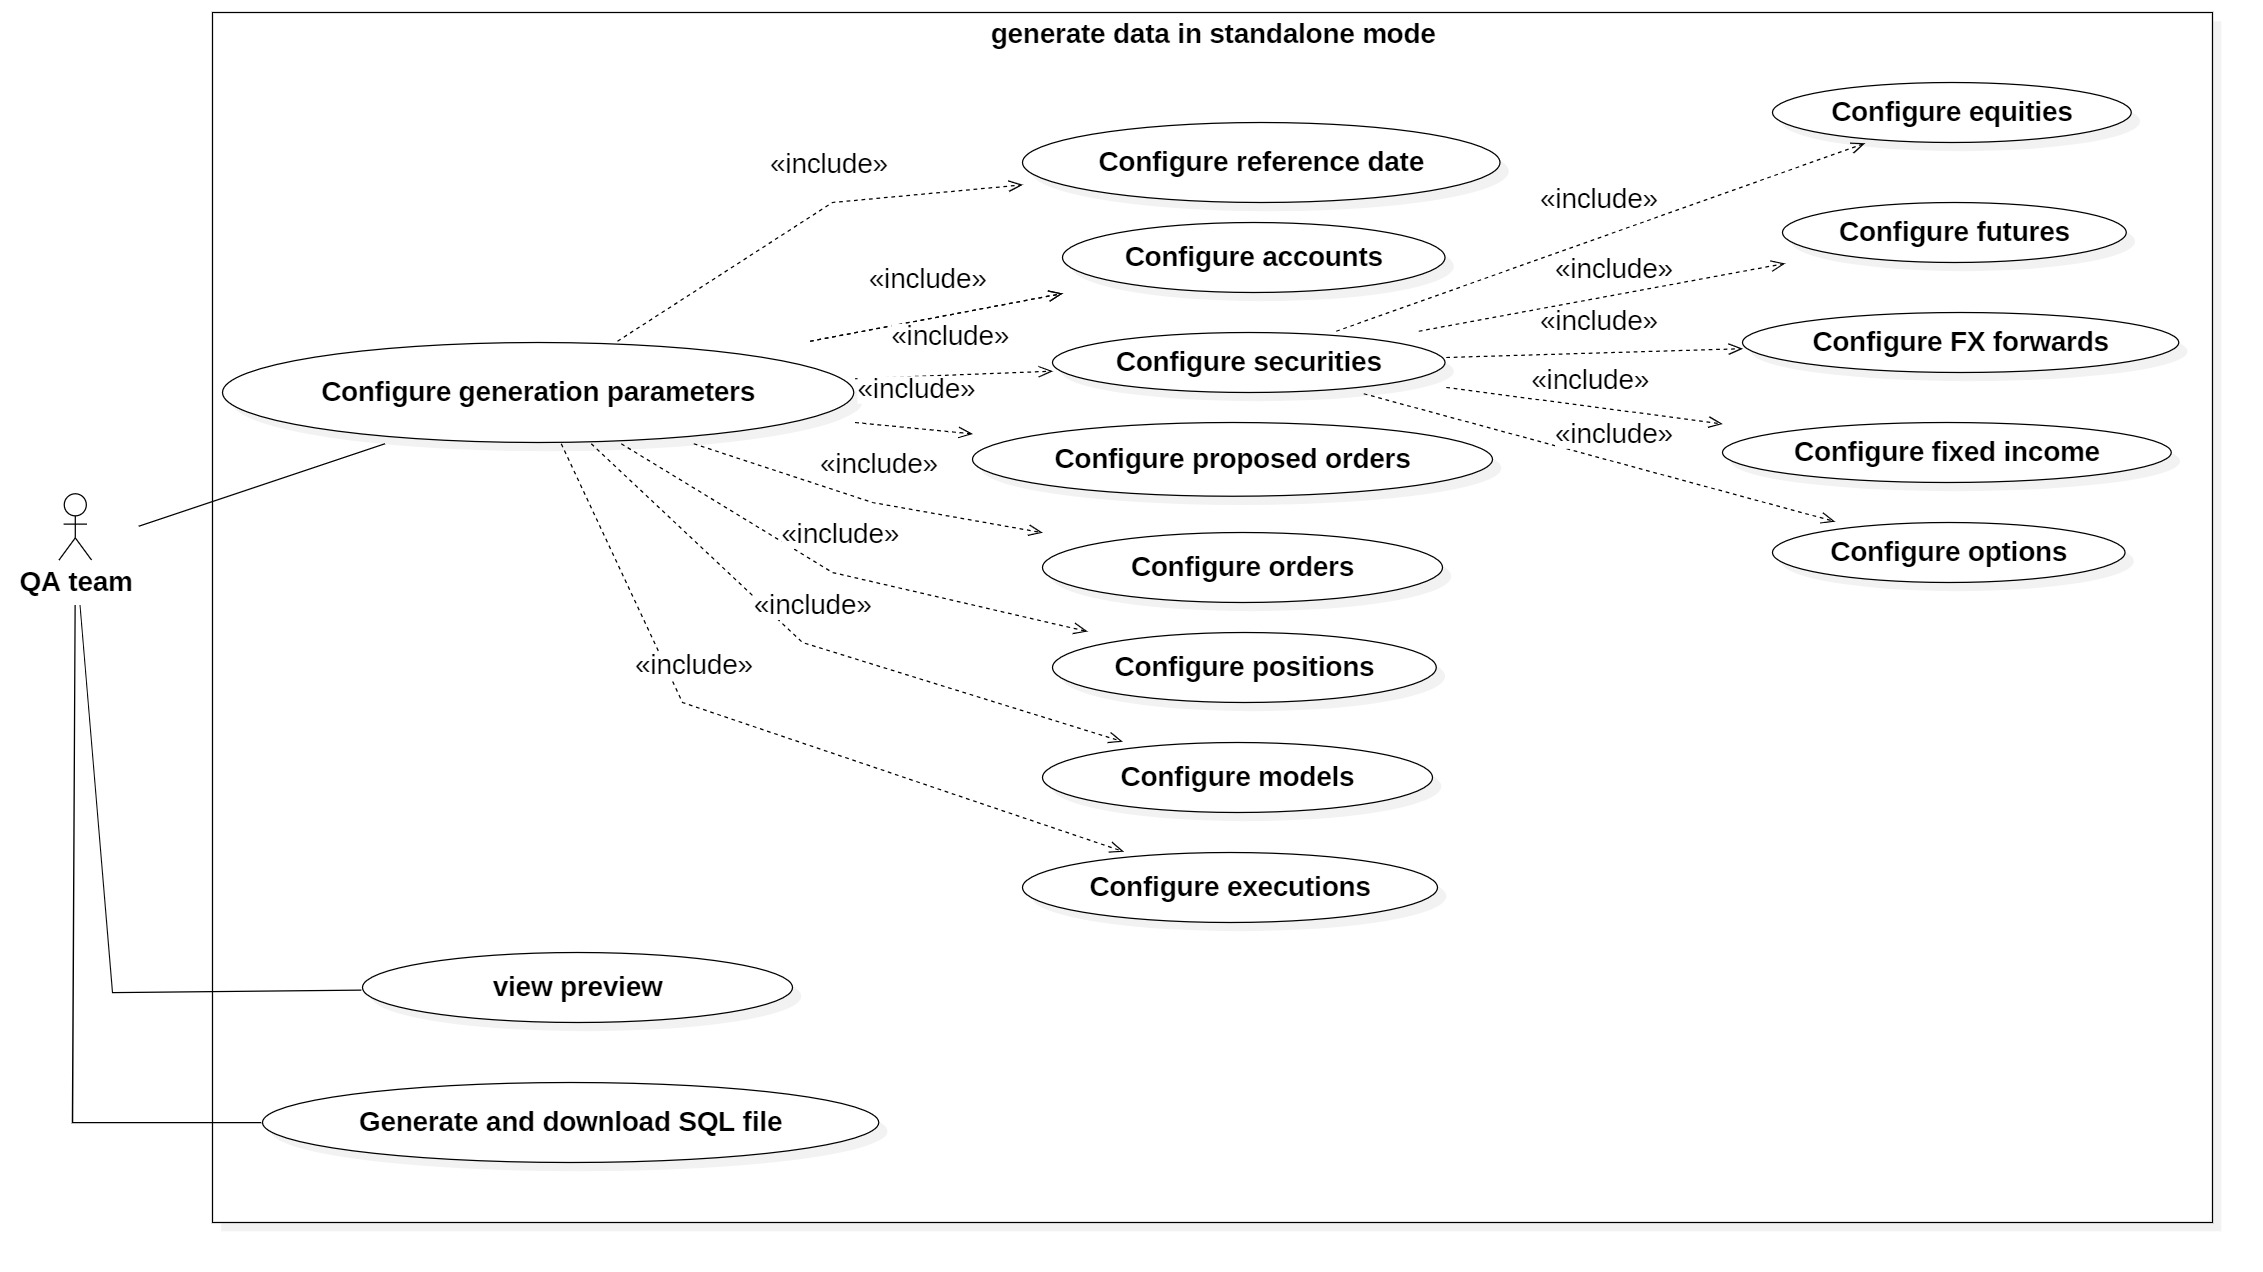
\includegraphics[width=0.95\textwidth]{img/usecase-standalone-mode-clean.jpg}
\caption{Refined use case diagram of standalone mode}
\label{fig:usecase-standalone}
\end{figure}

\renewcommand{\arraystretch}{1.15}
\begin{longtable}{|P{0.27\linewidth}|P{0.23\linewidth}|P{0.40\linewidth}|}
\caption{Refined use cases of Sprint 2}
\label{tab:sprint2-refined-usecases} \\
\hline
\textbf{Refined use case} & \textbf{Actor} & \textbf{Goal} \\
\hline
\endfirsthead
\multicolumn{3}{r}{\tablename\ \thetable{} -- \textit{continued from previous page}} \\
\hline
\textbf{Refined use case} & \textbf{Actor} & \textbf{Goal} \\
\hline
\endhead
\hline
\multicolumn{3}{r}{\textit{continued on next page}} \\
\endfoot
\hline
\endlastfoot
Configure generation parameters & QA Engineer & Define what data must be generated and with which quantities, ranges, ratios, and naming rules. \\
\hline
Configure reference date & QA Engineer & Set the base date used by prices, positions, orders, executions, and generated financial dates. \\
\hline
Configure accounts & QA Engineer & Generate the account universe used by models, positions, orders, and executions. \\
\hline
Configure securities & QA Engineer & Select the instrument types and quantities used by prices, positions, orders, models, and executions. \\
\hline
Configure proposed orders & QA Engineer & Generate proposed trades using accounts, securities, quantity ranges, and buy/sell ratio. \\
\hline
Configure orders & QA Engineer & Generate final orders that can later be used by executions. \\
\hline
Configure positions & QA Engineer & Generate holdings for account-security pairs, with long/short and tax-lot options. \\
\hline
Configure models & QA Engineer & Generate model allocations based on generated accounts and securities. \\
\hline
Configure executions & QA Engineer & Generate fills only when final orders are available. \\
\hline
View preview & QA Engineer & Review estimated record counts before launching generation. \\
\hline
Generate and download SQL script & QA Engineer & Produce and download the SQL Server loading script. \\
\hline
\end{longtable}
\renewcommand{\arraystretch}{1}

\subsection{Textual Use Case Description}

\subsubsection{Configure Generation Parameters}

\paragraph{}Table~\ref{tab:configure-generation-usecase} details the configuration use case and the
guards applied before preview.

\renewcommand{\arraystretch}{1.15}
\begin{longtable}{|P{0.24\linewidth}|P{0.66\linewidth}|}
\caption{Textual description of the configuration use case}
\label{tab:configure-generation-usecase} \\
\hline
\textbf{Element} & \textbf{Description} \\
\hline
\endfirsthead
\multicolumn{2}{r}{\tablename\ \thetable{} -- \textit{continued from previous page}} \\
\hline
\textbf{Element} & \textbf{Description} \\
\hline
\endhead
\hline
\multicolumn{2}{r}{\textit{continued on next page}} \\
\endfoot
\hline
\endlastfoot
Use case & Configure generation parameters. \\
\hline
Actor & QA Engineer. \\
\hline
Preconditions & The QA engineer selected standalone mode and reached the configuration step. \\
\hline
Postconditions & A valid standalone configuration is available for preview and generation. \\
\hline
Main scenario &
\begin{enumerate}[leftmargin=*,nosep]
    \item The QA engineer chooses the reference date.
    \item The QA engineer enables account generation and defines the number of accounts, currency, and naming patterns.
    \item The QA engineer enables security generation and enters quantities for the selected instrument types.
    \item The QA engineer optionally enables proposed orders, final orders, positions, models, and executions.
    \item The system checks dependency rules, disables unavailable dependent sections, and reports invalid values.
    \item The system displays a summary of the selected configuration and enables the next step only when the configuration is valid.
\end{enumerate} \\
\hline
Configuration guards &
\begin{itemize}[leftmargin=*,nosep]
    \item At least one data family, accounts or securities, must be selected.
    \item Proposed orders, final orders, positions, models, and executions require both accounts and securities.
    \item Executions require final orders.
    \item Fixed-income schedules are available only when fixed-income securities are selected.
    \item Quantity and value maximums must be greater than or equal to their minimums.
    \item Generation quantities must remain within the frontend and backend safety limits.
    \item Estimated output above 100,000 rows raises a warning, while output above 500,000 rows blocks generation.
    \item Tax lots require at least two lots per position.
\end{itemize} \\
\hline
Exception scenario &
\begin{itemize}[leftmargin=*,nosep]
    \item If no data is selected, the system displays validation messages and blocks access to preview.
    \item If accounts or securities are not available, the dependent sections are disabled and any already selected dependent options are cleared.
    \item If orders are disabled while executions are enabled, executions are automatically disabled.
    \item If invalid numeric values are entered, the system displays validation messages and blocks access to preview.
    \item If the estimated output exceeds the maximum row budget, the system blocks preview or generation until the configuration is reduced.
\end{itemize} \\
\hline
\end{longtable}
\renewcommand{\arraystretch}{1}

\subsubsection{View Preview}

\paragraph{}Table~\ref{tab:preview-usecase} describes the preview step used to review the estimated
generation result before launching the backend process.

\renewcommand{\arraystretch}{1.15}
\begin{longtable}{|P{0.24\linewidth}|P{0.66\linewidth}|}
\caption{Textual description of the preview use case}
\label{tab:preview-usecase} \\
\hline
\textbf{Element} & \textbf{Description} \\
\hline
\endfirsthead
\multicolumn{2}{r}{\tablename\ \thetable{} -- \textit{continued from previous page}} \\
\hline
\textbf{Element} & \textbf{Description} \\
\hline
\endhead
\hline
\multicolumn{2}{r}{\textit{continued on next page}} \\
\endfoot
\hline
\endlastfoot
Use case & View preview. \\
\hline
Actor & QA Engineer. \\
\hline
Preconditions & The standalone configuration is valid. \\
\hline
Postconditions & The QA engineer can decide whether to return to configuration or launch generation. \\
\hline
Main scenario &
\begin{enumerate}[leftmargin=*,nosep]
    \item The QA engineer opens the preview step.
    \item The frontend estimates generated records from account count, security quantities, selected dependencies, and per-account options.
    \item The system displays a summary of the expected generation result, including the target buffer table and loading procedure for each generated data category.
    \item The QA engineer either returns to configuration or starts generation.
\end{enumerate} \\
\hline
Exception scenario & If the configuration contains missing dependencies or invalid values, the
system disables access to the preview and displays the corresponding validation messages in the
configuration summary. The QA engineer corrects the affected parameters before opening the preview. \\
\hline
\end{longtable}
\renewcommand{\arraystretch}{1}

\subsubsection{Generate and Download SQL Script}

\paragraph{}Table~\ref{tab:generate-sql-usecase} describes the final generation step, from backend
execution to SQL download.

\renewcommand{\arraystretch}{1.15}
\begin{longtable}{|P{0.24\linewidth}|P{0.66\linewidth}|}
\caption{Textual description of the SQL generation use case}
\label{tab:generate-sql-usecase} \\
\hline
\textbf{Element} & \textbf{Description} \\
\hline
\endfirsthead
\multicolumn{2}{r}{\tablename\ \thetable{} -- \textit{continued from previous page}} \\
\hline
\textbf{Element} & \textbf{Description} \\
\hline
\endhead
\hline
\multicolumn{2}{r}{\textit{continued on next page}} \\
\endfoot
\hline
\endlastfoot
Use case & Generate and download SQL script. \\
\hline
Actor & QA Engineer. \\
\hline
Preconditions & The QA engineer validated the preview and launched generation. \\
\hline
Postconditions & A SQL Server loading script is downloaded if generation and validation succeed. \\
\hline
Main scenario &
\begin{enumerate}[leftmargin=*,nosep]
    \item The frontend sends the standalone configuration to the backend.
    \item The backend normalizes the reference date and prepares a generation run.
    \item The backend generates the requested financial domains in dependency order.
    \item The backend validates required fields and references between generated records.
    \item The backend assembles the SQL loading script in the expected loading order.
    \item The frontend displays user-friendly real-time logs showing the generation progress, the generated data categories, and any warning or error encountered.
    \item The frontend downloads the SQL file and displays the generation summary.
\end{enumerate} \\
\hline
Exception scenario &
\begin{itemize}[leftmargin=*,nosep]
    \item If backend generation, relationship validation, generated-record validation, SQL assembly, or file download fails, the generation run is marked as failed.
    \item The frontend displays the returned error message in the generation step, keeps the generation log available, and does not mark the run as successful.
\end{itemize} \\
\hline
\end{longtable}
\renewcommand{\arraystretch}{1}

\section{Sprint Design}

\paragraph{}The design of Sprint 2 connects the standalone interface with the internal generation engine.
The frontend owns the user workflow and first-level configuration checks. The backend owns the
generation algorithm, final validation, and SQL assembly.

\subsection{Sequence Diagrams}

\paragraph{}Figure~\ref{fig:sequence-standalone} presents the frontend and backend exchanges of the
standalone sequence.

\begin{figure}[!htbp]
\centering
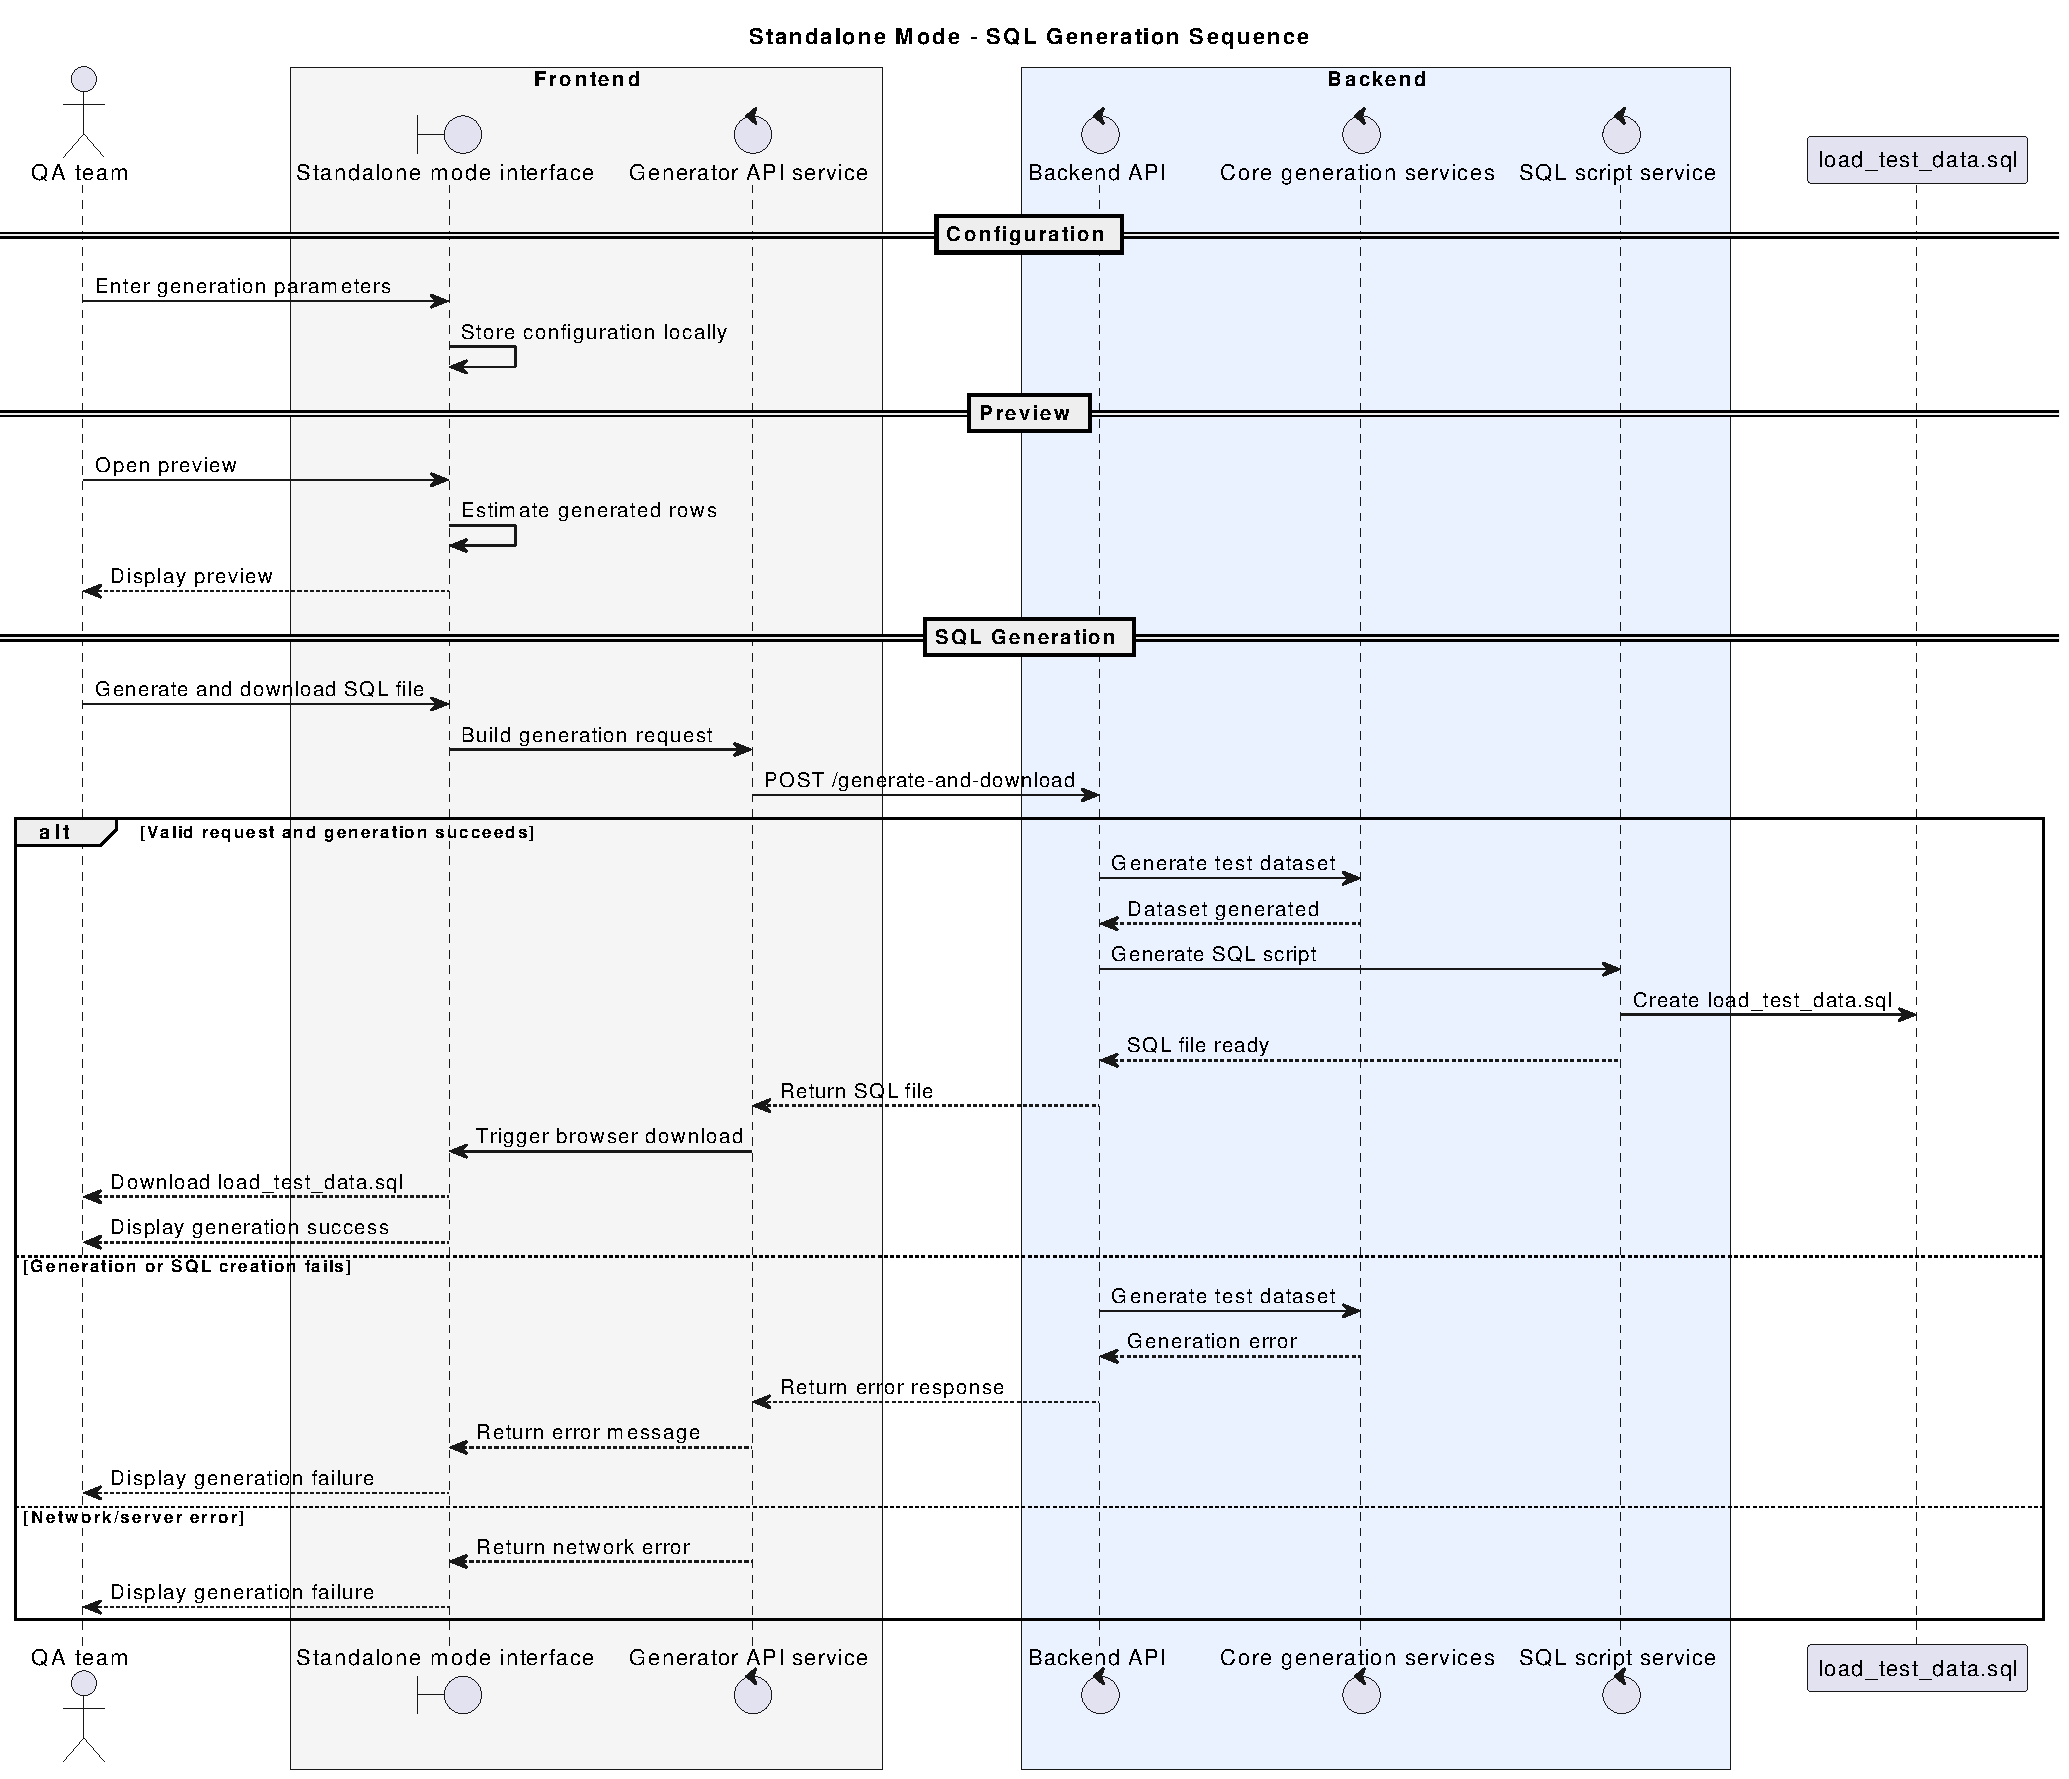
\includegraphics[width=0.95\textwidth]{img/sequence-standalone-mode.pdf}
\caption{Standalone mode SQL generation sequence}
\label{fig:sequence-standalone}
\end{figure}

\subsection{Backend Workflow Diagram}

\paragraph{}Figure~\ref{fig:ch4-backend-standalone-workflow} presents the backend workflow followed after
the QA engineer launches standalone generation.

\begin{figure}[!htbp]
\centering
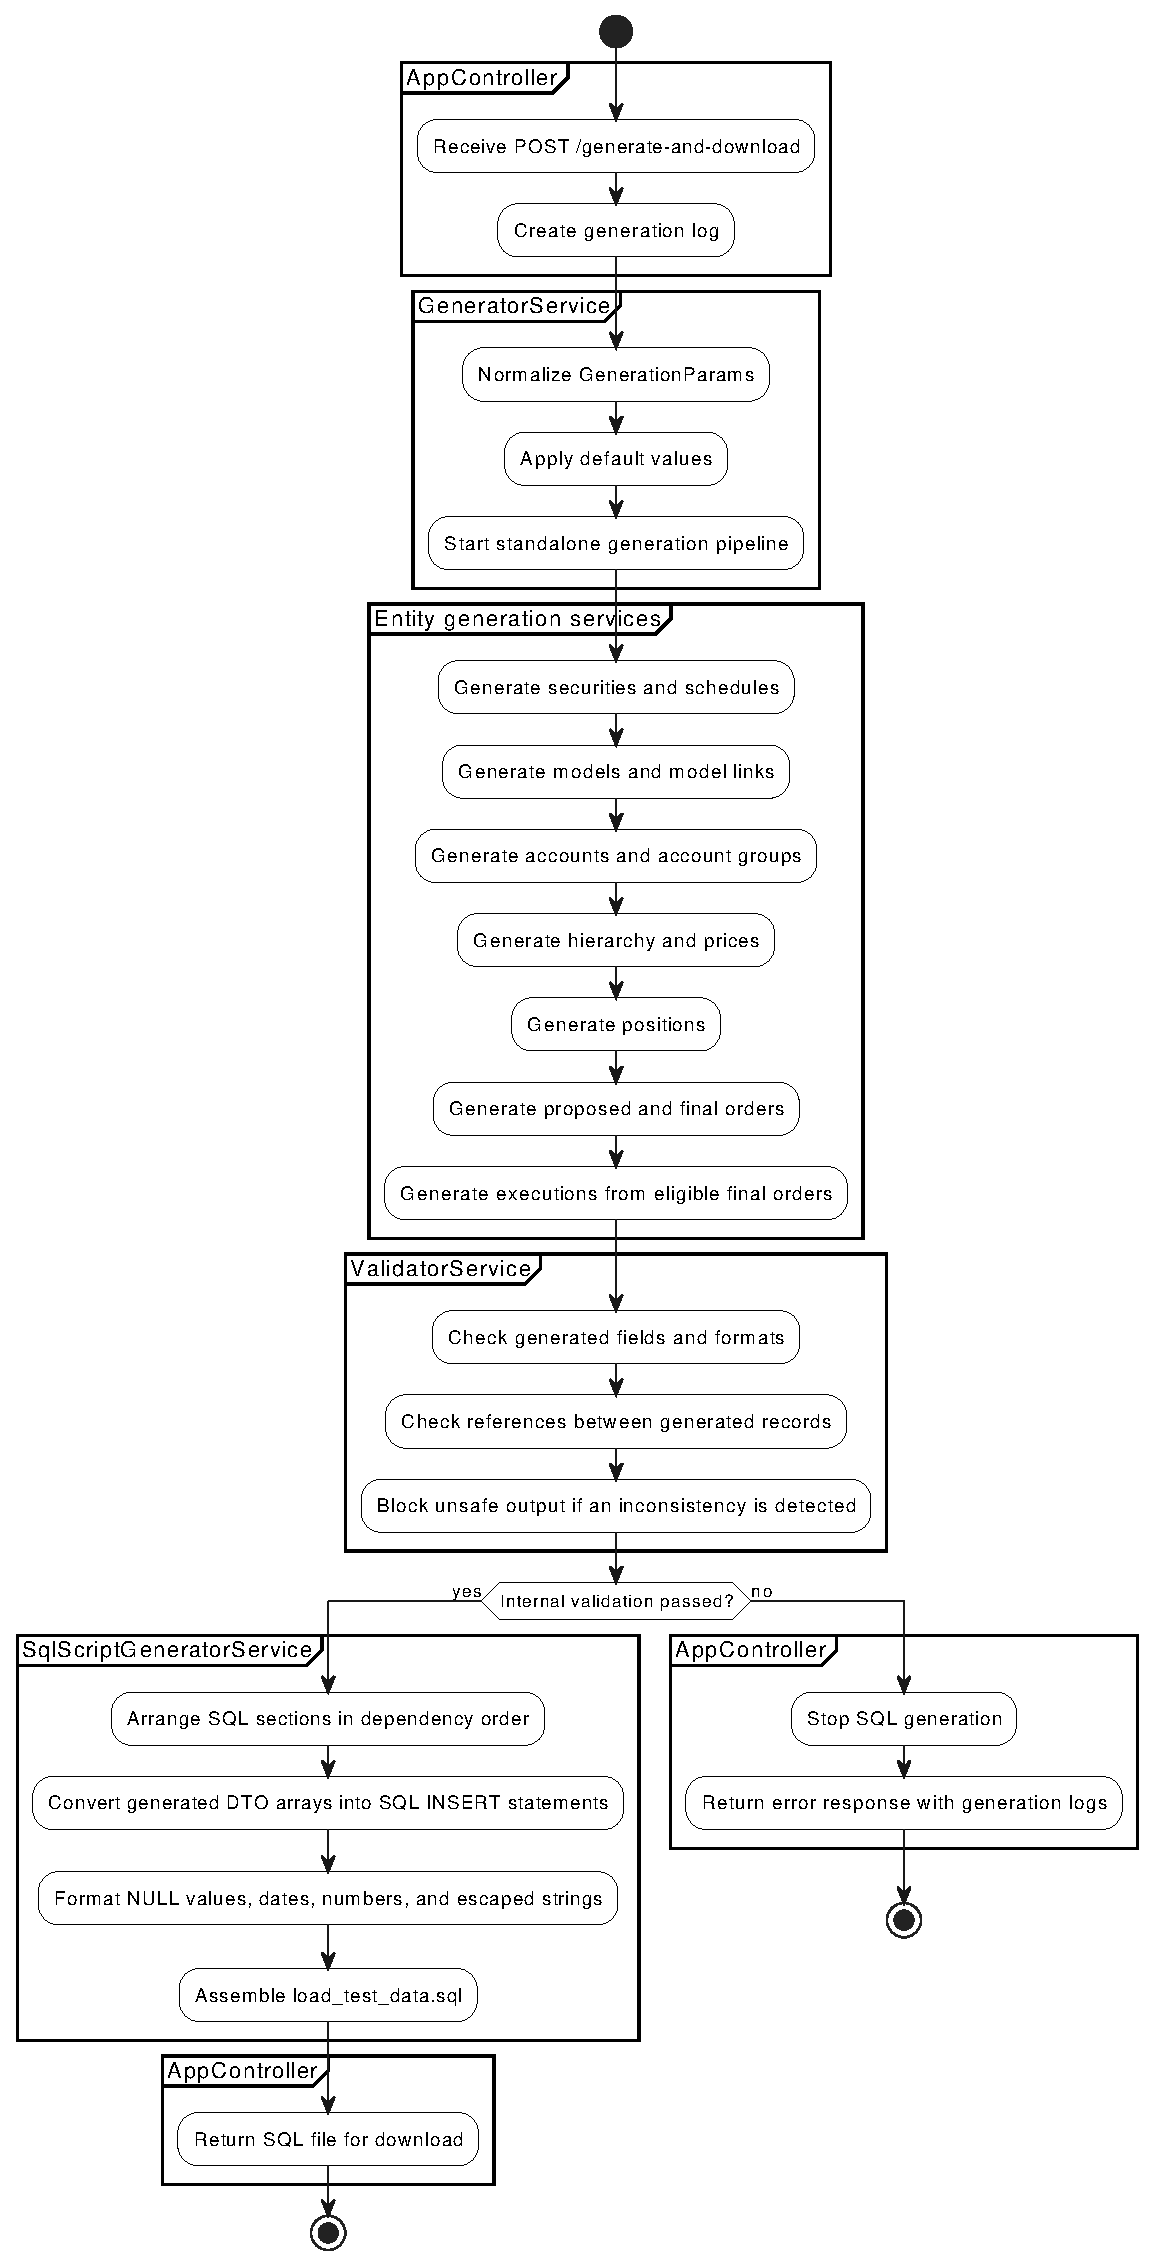
\includegraphics[width=0.95\textwidth,height=0.78\textheight,keepaspectratio]{img/ch4-backend-standalone-workflow.pdf}
\caption{Backend standalone SQL generation workflow}
\label{fig:ch4-backend-standalone-workflow}
\end{figure}

\section{Realization}

\subsection{Configuration Parameters}

\paragraph{}The standalone configuration page is implemented by \texttt{StandaloneConfigurationTab.tsx}
and shared configuration components. Table~\ref{tab:standalone-config-mapping} maps each section to
its main generation effect.

\renewcommand{\arraystretch}{1.12}
\begin{longtable}{|P{0.22\linewidth}|P{0.38\linewidth}|P{0.30\linewidth}|}
\caption{Standalone configuration mapping}
\label{tab:standalone-config-mapping} \\
\hline
\textbf{Section} & \textbf{Main inputs} & \textbf{Effect on generation} \\
\hline
\endfirsthead
\multicolumn{3}{r}{\tablename\ \thetable{} -- \textit{continued from previous page}} \\
\hline
\textbf{Section} & \textbf{Main inputs} & \textbf{Effect on generation} \\
\hline
\endhead
\hline
\multicolumn{3}{r}{\textit{continued on next page}} \\
\endfoot
\hline
\endlastfoot
Reference date & Base date selected from the date picker & Controls generated business dates such as prices, order dates, settlement dates, and execution dates. \\
\hline
Accounts & Enable flag, count (max: 5,000), currency, short name pattern, long name pattern & Creates the account universe used by dependent portfolio and trading data. \\
\hline
Securities & Enable flag and quantities for equity, fixed income, futures, options, FX forwards, and generic securities (max: 10,000 for equities, fixed income, and options; 5,000 for futures, FX forwards, and generics) & Creates the instrument universe used by prices, positions, orders, executions, and models. \\
\hline
Fixed-income schedules & CALL, PUT, COUP, and CONVERT rows per eligible fixed-income security (max: 20) & Adds optional schedule details for selected fixed-income instruments. \\
\hline
Proposed orders & Orders per account (max: 100), quantity range, buy/sell ratio & Creates proposed trade requests anchored to generated accounts and securities. \\
\hline
Final orders & Orders per account (max: 100), quantity range, buy/sell ratio & Creates order records that can be used by execution generation. \\
\hline
Positions & Positions per account (max: 100), long/short ratio, quantity range, value range, tax-lot option, tax lots per position (max: 10) & Creates account-security holdings and optional tax-lot splits. \\
\hline
Models & Models per account (max: 5), allocation mode, minimum allocation percentage & Creates model allocations using generated accounts and securities. \\
\hline
Executions & Executions per order (max: 5), partial fill percentage, commission rate type, commission rate & Creates fills for eligible generated orders. \\
\hline
\end{longtable}
\renewcommand{\arraystretch}{1}

\subsection{Preview Estimation}

\paragraph{}The preview is calculated on the frontend from the current configuration, without running
the backend generation algorithm. Table~\ref{tab:preview-estimation-rules} summarizes the main
estimation rules.

\renewcommand{\arraystretch}{1.15}
\begin{longtable}{|P{0.26\linewidth}|P{0.34\linewidth}|P{0.30\linewidth}|}
\caption{Preview estimation rules}
\label{tab:preview-estimation-rules} \\
\hline
\textbf{Estimated data} & \textbf{Formula or rule} & \textbf{Condition} \\
\hline
\endfirsthead
\multicolumn{3}{r}{\tablename\ \thetable{} -- \textit{continued from previous page}} \\
\hline
\textbf{Estimated data} & \textbf{Formula or rule} & \textbf{Condition} \\
\hline
\endhead
\hline
\multicolumn{3}{r}{\textit{continued on next page}} \\
\endfoot
\hline
\endlastfoot
Accounts & Account count & Account generation is enabled. \\
\hline
Securities & Sum of selected security subtype quantities & Security generation is enabled. \\
\hline
Prices & One price per generated security & At least one security is selected. \\
\hline
Positions & Accounts multiplied by positions per account, limited by available tradable securities & Positions are enabled and the configuration is valid. \\
\hline
Proposed orders & Accounts multiplied by proposed orders per account & Proposed orders are enabled and the configuration is valid. \\
\hline
Final orders & Accounts multiplied by orders per account & Orders are enabled and the configuration is valid. \\
\hline
Executions & Estimated equity orders multiplied by executions per order & Executions and orders are enabled. \\
\hline
Models & Accounts multiplied by models per account and allocation rows per model & Models are enabled and the configuration is valid. \\
\hline
\end{longtable}
\renewcommand{\arraystretch}{1}

\subsection{Internal Generation Algorithm}

\paragraph{}At this stage, the standalone data is generated by the application's internal algorithms.
The generated records are not taken from an existing database or from external input files. Instead,
the backend creates the requested accounts, securities, prices, positions, orders, executions, and
related records from the configuration entered by the QA engineer. It relies on predefined templates
and code lists stored in the backend, then applies controlled pseudo-random variation to generate
different names, quantities, prices, dates, and trading values while preserving the required links
between records.


\subsection{User Workflow}

\paragraph{}The following figures show the implemented standalone screens. Their routing and state
transitions are managed by \texttt{StandaloneMode.tsx}.

\paragraph{}Figure~\ref{fig:ch4-mode-selection} shows the entry screen where the user selects the
standalone mode.

\begin{figure}[!htbp]
\centering
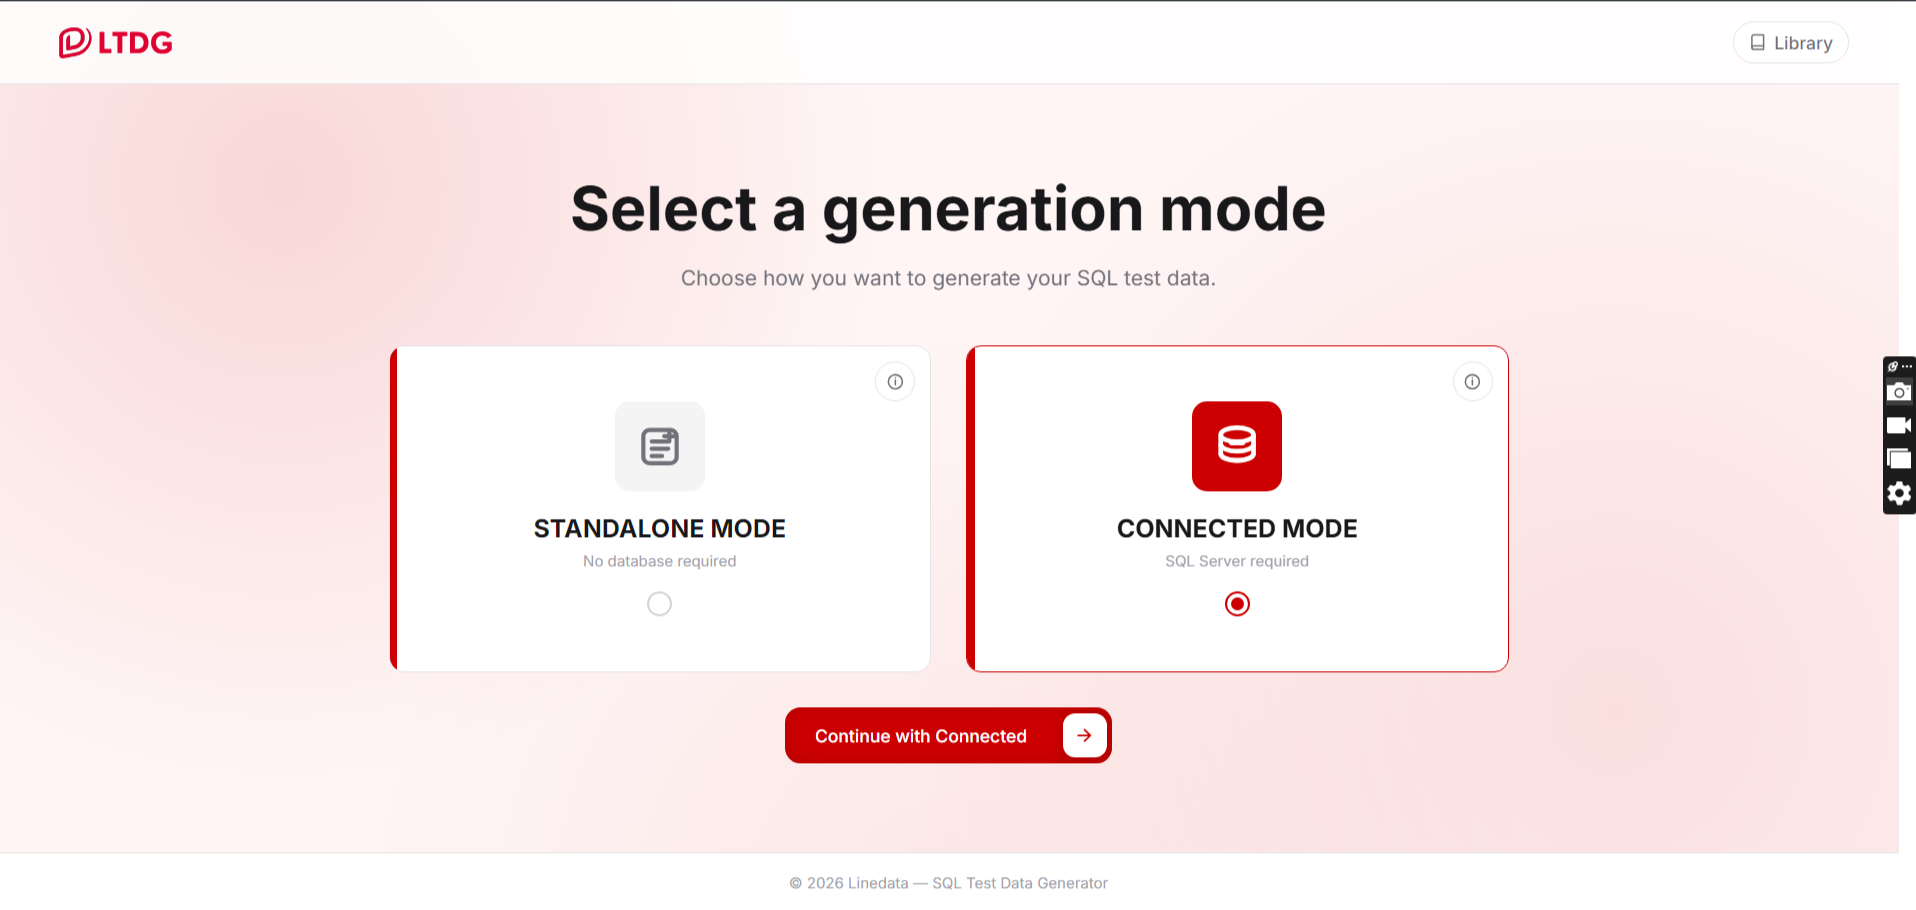
\includegraphics[width=0.88\textwidth]{img/ch4-mode-selection.png}
\caption{Mode selection screen}
\label{fig:ch4-mode-selection}
\end{figure}

\paragraph{}Figure~\ref{fig:ch4-step-config} shows the configuration screen where the QA engineer
defines the generation scope and the main parameters used by the backend.

\begin{figure}[!htbp]
\centering
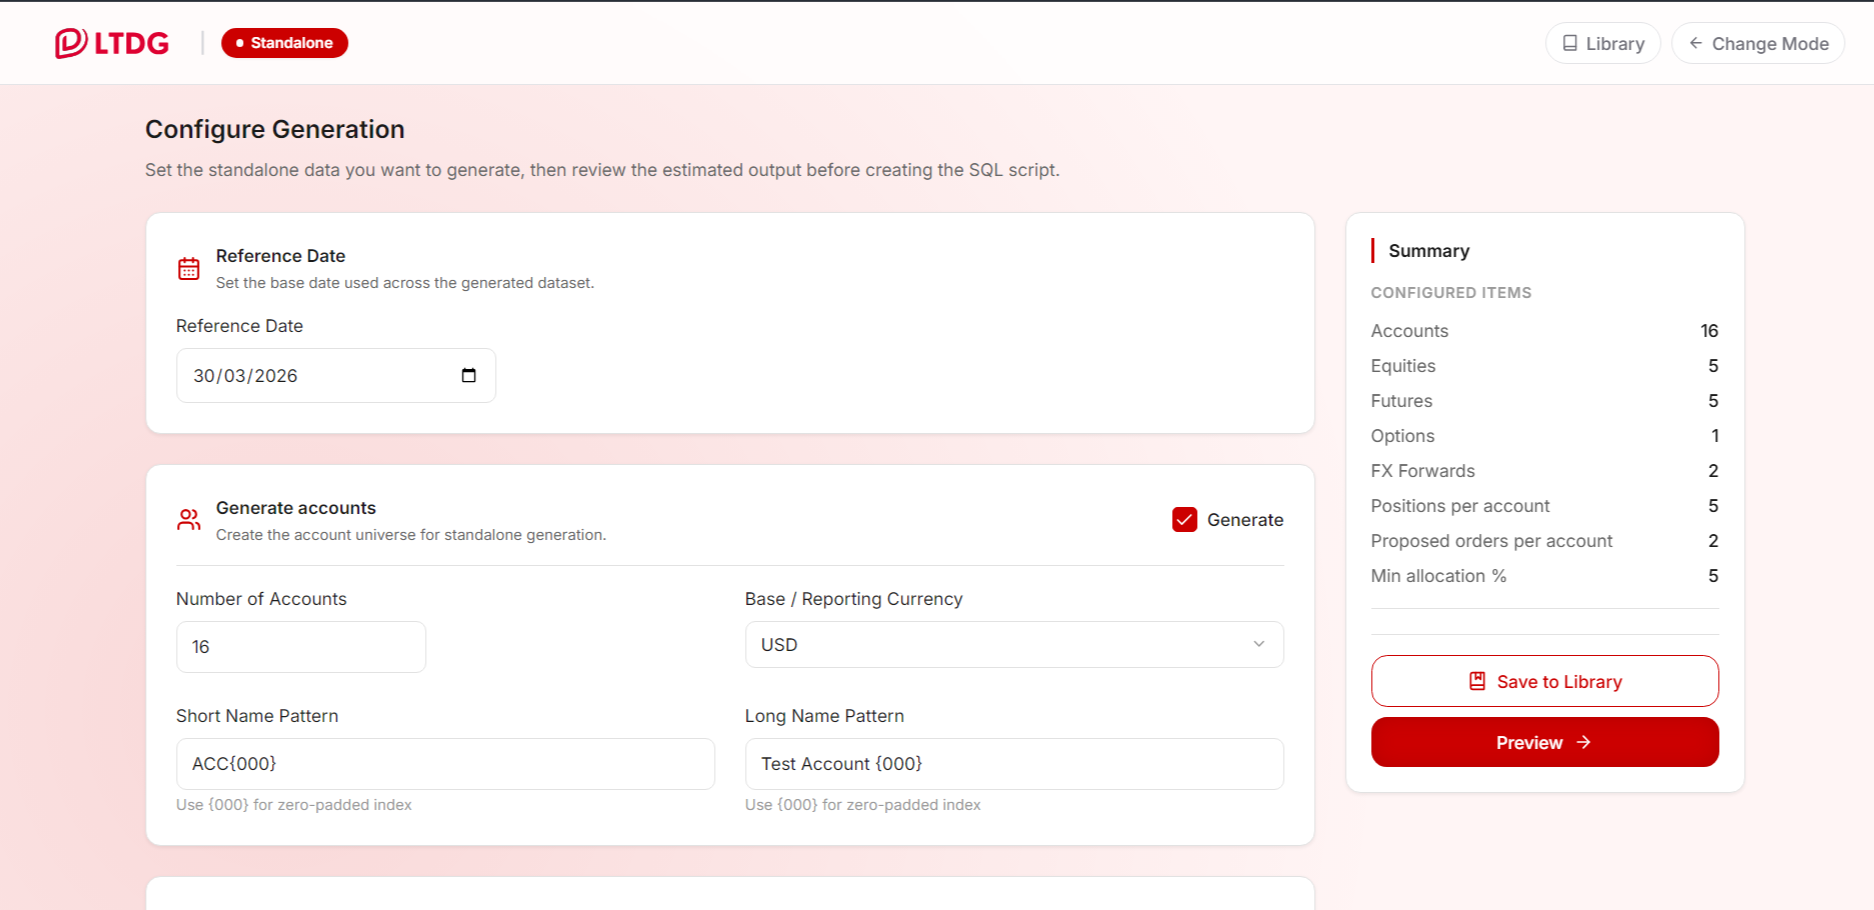
\includegraphics[width=0.88\textwidth]{img/ch4-step1-config.png}
\caption{Standalone configuration screen}
\label{fig:ch4-step-config}
\end{figure}

\paragraph{}Figure~\ref{fig:ch4-step-preview} shows the preview screen that summarizes the expected
result before the SQL generation request is launched.

\begin{figure}[!htbp]
\centering
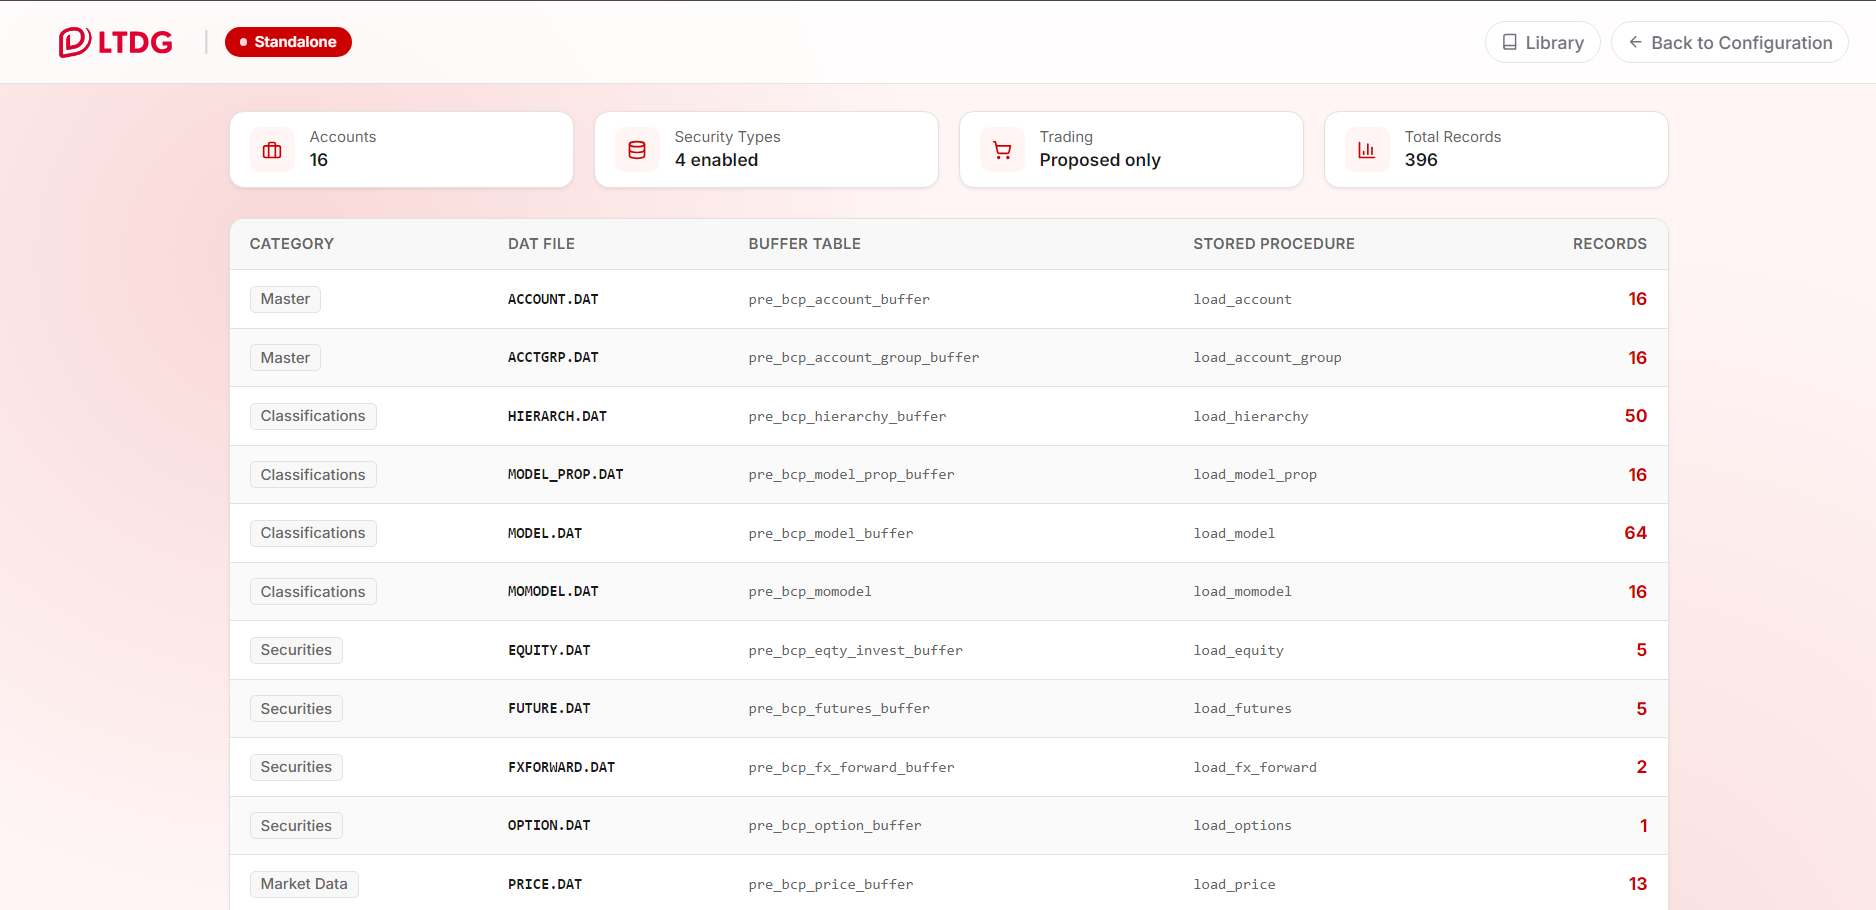
\includegraphics[width=0.88\textwidth]{img/ch4-step2-preview.png}
\caption{Standalone preview screen}
\label{fig:ch4-step-preview}
\end{figure}

\paragraph{}Figure~\ref{fig:ch4-step-result} shows the result screen displayed after generation, with
the execution status and access to the generated SQL script.

\begin{figure}[!htbp]
\centering
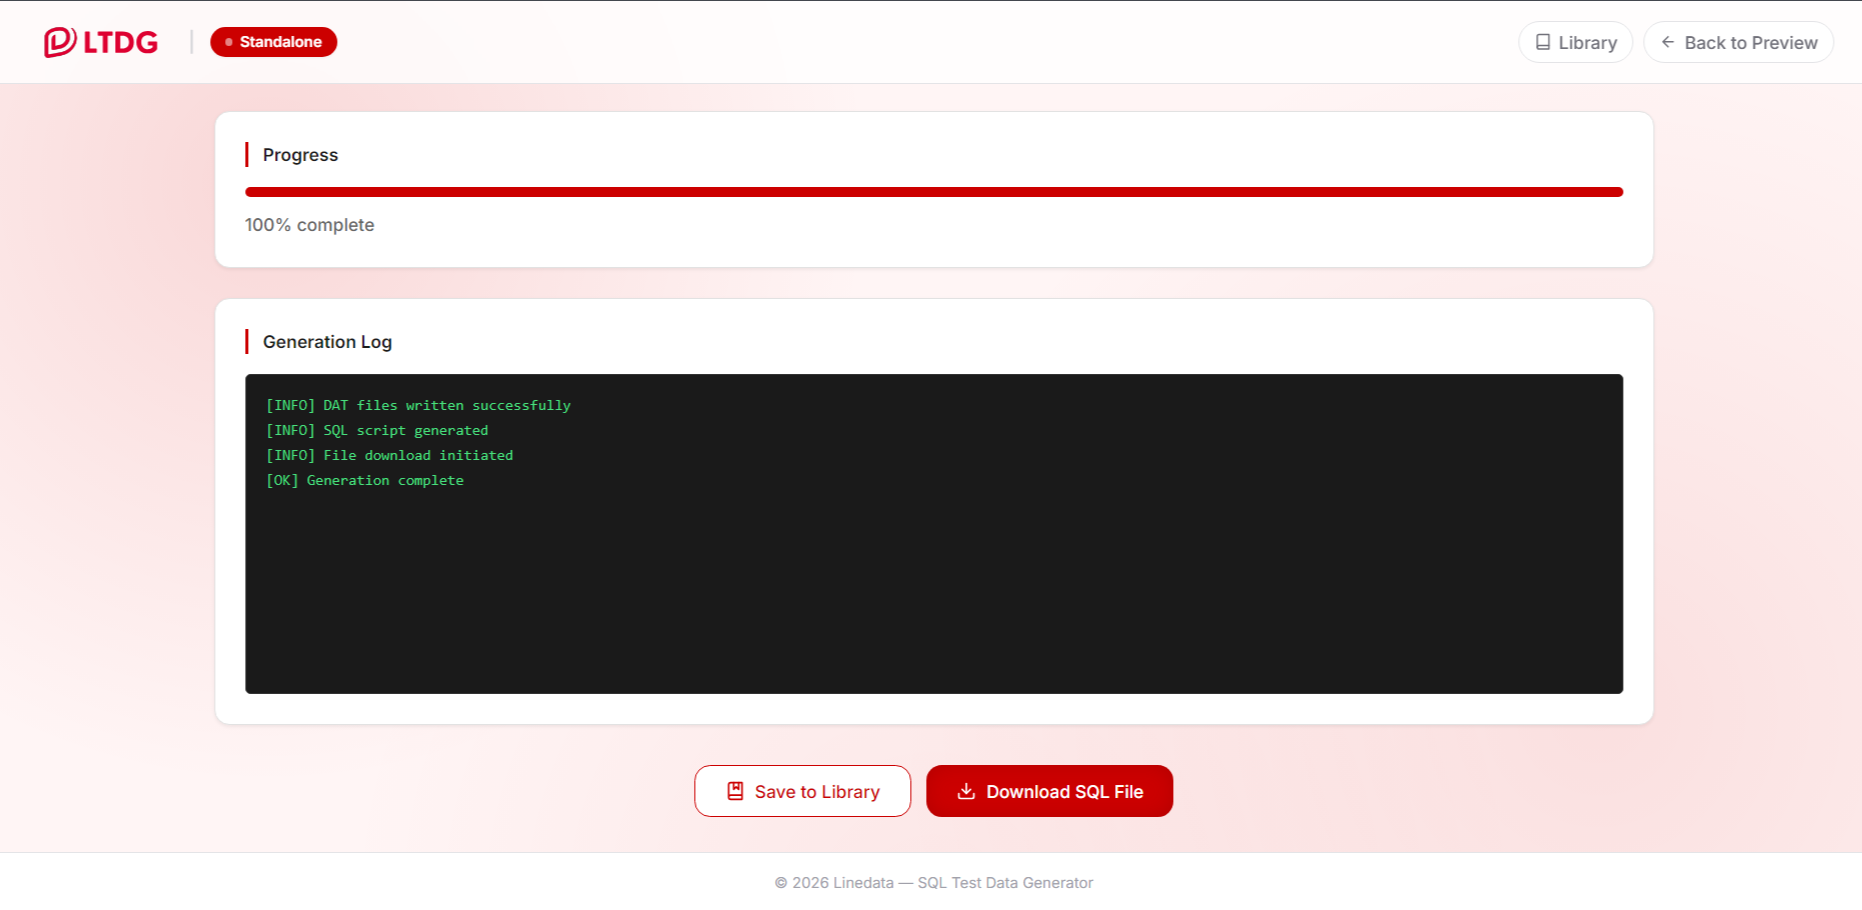
\includegraphics[width=0.88\textwidth]{img/ch4-step3-result.png}
\caption{Standalone generation result}
\label{fig:ch4-step-result}
\end{figure}

\subsection{Generated Output Evidence}

\paragraph{}After the QA engineer launches generation, the backend produces the configured
\texttt{.DAT} files, validates their field formats and relationships, and converts the validated output
into a SQL Server loading script. Table~\ref{tab:standalone-realization-proof} summarizes the main
realization evidence of this sprint.

\Needspace{12\baselineskip}
\renewcommand{\arraystretch}{1.3}
\begin{longtable}{|P{0.25\linewidth}|P{0.35\linewidth}|P{0.30\linewidth}|}
\caption{Standalone generation realization evidence}
\label{tab:standalone-realization-proof} \\
\hline
\textbf{Evidence} & \textbf{Implemented result} & \textbf{Purpose} \\
\hline
\endfirsthead
\multicolumn{3}{r}{\tablename\ \thetable{} -- \textit{continued from previous page}} \\
\hline
\textbf{Evidence} & \textbf{Implemented result} & \textbf{Purpose} \\
\hline
\endhead
\hline
\multicolumn{3}{r}{\textit{continued on next page}} \\
\endfoot
\hline
\endlastfoot
Generated files & The backend writes files such as \texttt{ACCOUNT.DAT}, \texttt{EQUITY.DAT}, \texttt{PRICE.DAT}, \texttt{POSITION.DAT}, \texttt{ORDER.DAT}, and \texttt{EXECUTION.DAT}. & Proves that the configuration is transformed into concrete Longview loading artifacts. \\
\hline
Field validation & Each generated file is checked against required fields, numeric fields, date formats, lengths, and flag values. & Prevents malformed rows from being exported. \\
\hline
Relationship validation & Accounts, securities, prices, positions, orders, executions, and models are checked before writing the final output. & Ensures that generated records reference existing generated entities. \\
\hline
SQL script generation & The validated \texttt{.DAT} files are converted into \texttt{load\_test\_data.sql}. & Provides a single SQL Server script that can be downloaded and executed by the QA engineer. \\
\hline
Generation feedback & The interface displays progress, warning, success, and error messages during the run. & Gives the user visibility over the generation process and its result. \\
\hline
\end{longtable}
\renewcommand{\arraystretch}{1}

\paragraph{}Figure~\ref{fig:ch4-generation-proof} can be completed later with a screenshot of the
generation log, the produced \texttt{.DAT} files, or a short excerpt from the generated SQL script.

\begin{figure}[!htbp]
\centering
\IfFileExists{img/ch4-generation-proof.png}{%
    \includegraphics[width=0.88\textwidth]{img/ch4-generation-proof.png}%
}{%
    \fbox{\parbox[c][0.22\textheight][c]{0.86\textwidth}{\centering Screenshot to be added: standalone generation log, generated DAT files, or SQL script excerpt}}%
}
\caption{Standalone generation output and validation evidence}
\label{fig:ch4-generation-proof}
\end{figure}

\section*{Conclusion}
\addcontentsline{toc}{section}{Conclusion}

\paragraph{}Sprint 2 delivered the first complete version of the test data generator through standalone
configuration, preview, generation, validation, and SQL export. This result prepares the transition
to the connected mode introduced in the next sprint.
